\section{Introduction}
	
There are four major objectives of this paper: (1) to describe in detail an alternative integrated statistical catch-age model (iSCAM), (2) examine parameter estimation performance using iSCAM, (3) perform a side-by-side comparison of the previous HCAM and iSCAM on the five major herring stocks, and (4) explore alternative assumptions about selectivity, catchability, and natural mortality using iSCAM.  The most recent assessment of BC herring stocks was conducted in 2010 using the Herring Catch Age Model (HCAMv2) which is documented in \cite{Clear2010}.  Furthermore, a review sponsored by the Herring Research and Conservation Society (HRCS) was conducted June 17-18, 2010 in Nanaimo, BC where an expert panel addressed specific questions about the current implementation of the HCAMv2 model and suggested recommendations for each of the questions.  This paper also attempts to address some of the points brought up in the review.

BC herring are currently managed as five major stocks and 2 minor stocks (Figure \ref{Fig1}).  Annual catch advice for each of these areas is based on current estimates of stock status, and a 20\% exploitation rate if the stock is above the cutoff level for the five major stocks and a 10\% exploitation rate for the two minor stocks.  Cutoff levels for the five major stocks are based on 0.25$B_o$, and estimates of unfished biomass were established first in 1985 \citep{haist1986stock}.  These cutoffs are currently are thought to be more conservative 	than the current default Limit Reference Point of 0.4\bmsy\ \citep{dfo2006}. However, estimates of $B_o$ and MSY based reference points have not been examined for Pacific herring for some time.  In this paper we also describe the methods for updating estimates of $B_o$ and MSY based reference points using the iSCAM model framework.  We also compare estimates of MSY based reference points for the Strait of Georgia herring under the previously mentioned alternative assumptions (see point (4) in the previous paragraph).

We do not provide a detailed description of HCAMv2 in this paper and we refer the reader to \cite{schweigert2009stock} and \cite{Clear2010} for a more detailed description.  We first begin with a description of the input data required and assumptions about the data, followed by a detailed description of the analytical methods and assumptions in iSCAM. We then present the analytical methods and assumptions for exploring alternative hypotheses about selectivity, catchability and natural mortality, followed by a description of the elements that make up the joint posterior distribution (i.e., likelihoods, priors, and penalties).  Parameter estimating and quantifying uncertainty is carried out using AD Model Builder \citep{ADMB2009}.  We then explore estimation performance in iSCAM using simulation experiments where the model is used to generate simulated observations with known parameter values, then estimate parameter, and repeat this exercise a number of times to evaluate bias and precision in parameter estimates.  Finally, we present forecast of pre-fishery biomass and available harvest options using the cutoffs \cite[e.g., reproduce Table 5 in ][]{Clear2010} as well as available harvest options based on the Sustainable Fisheries Framework \citep[i.e.,][]{dfo2006} for comparison.

\begin{figure}[!tbp]
	% Requires \usepackage{graphicx}
	%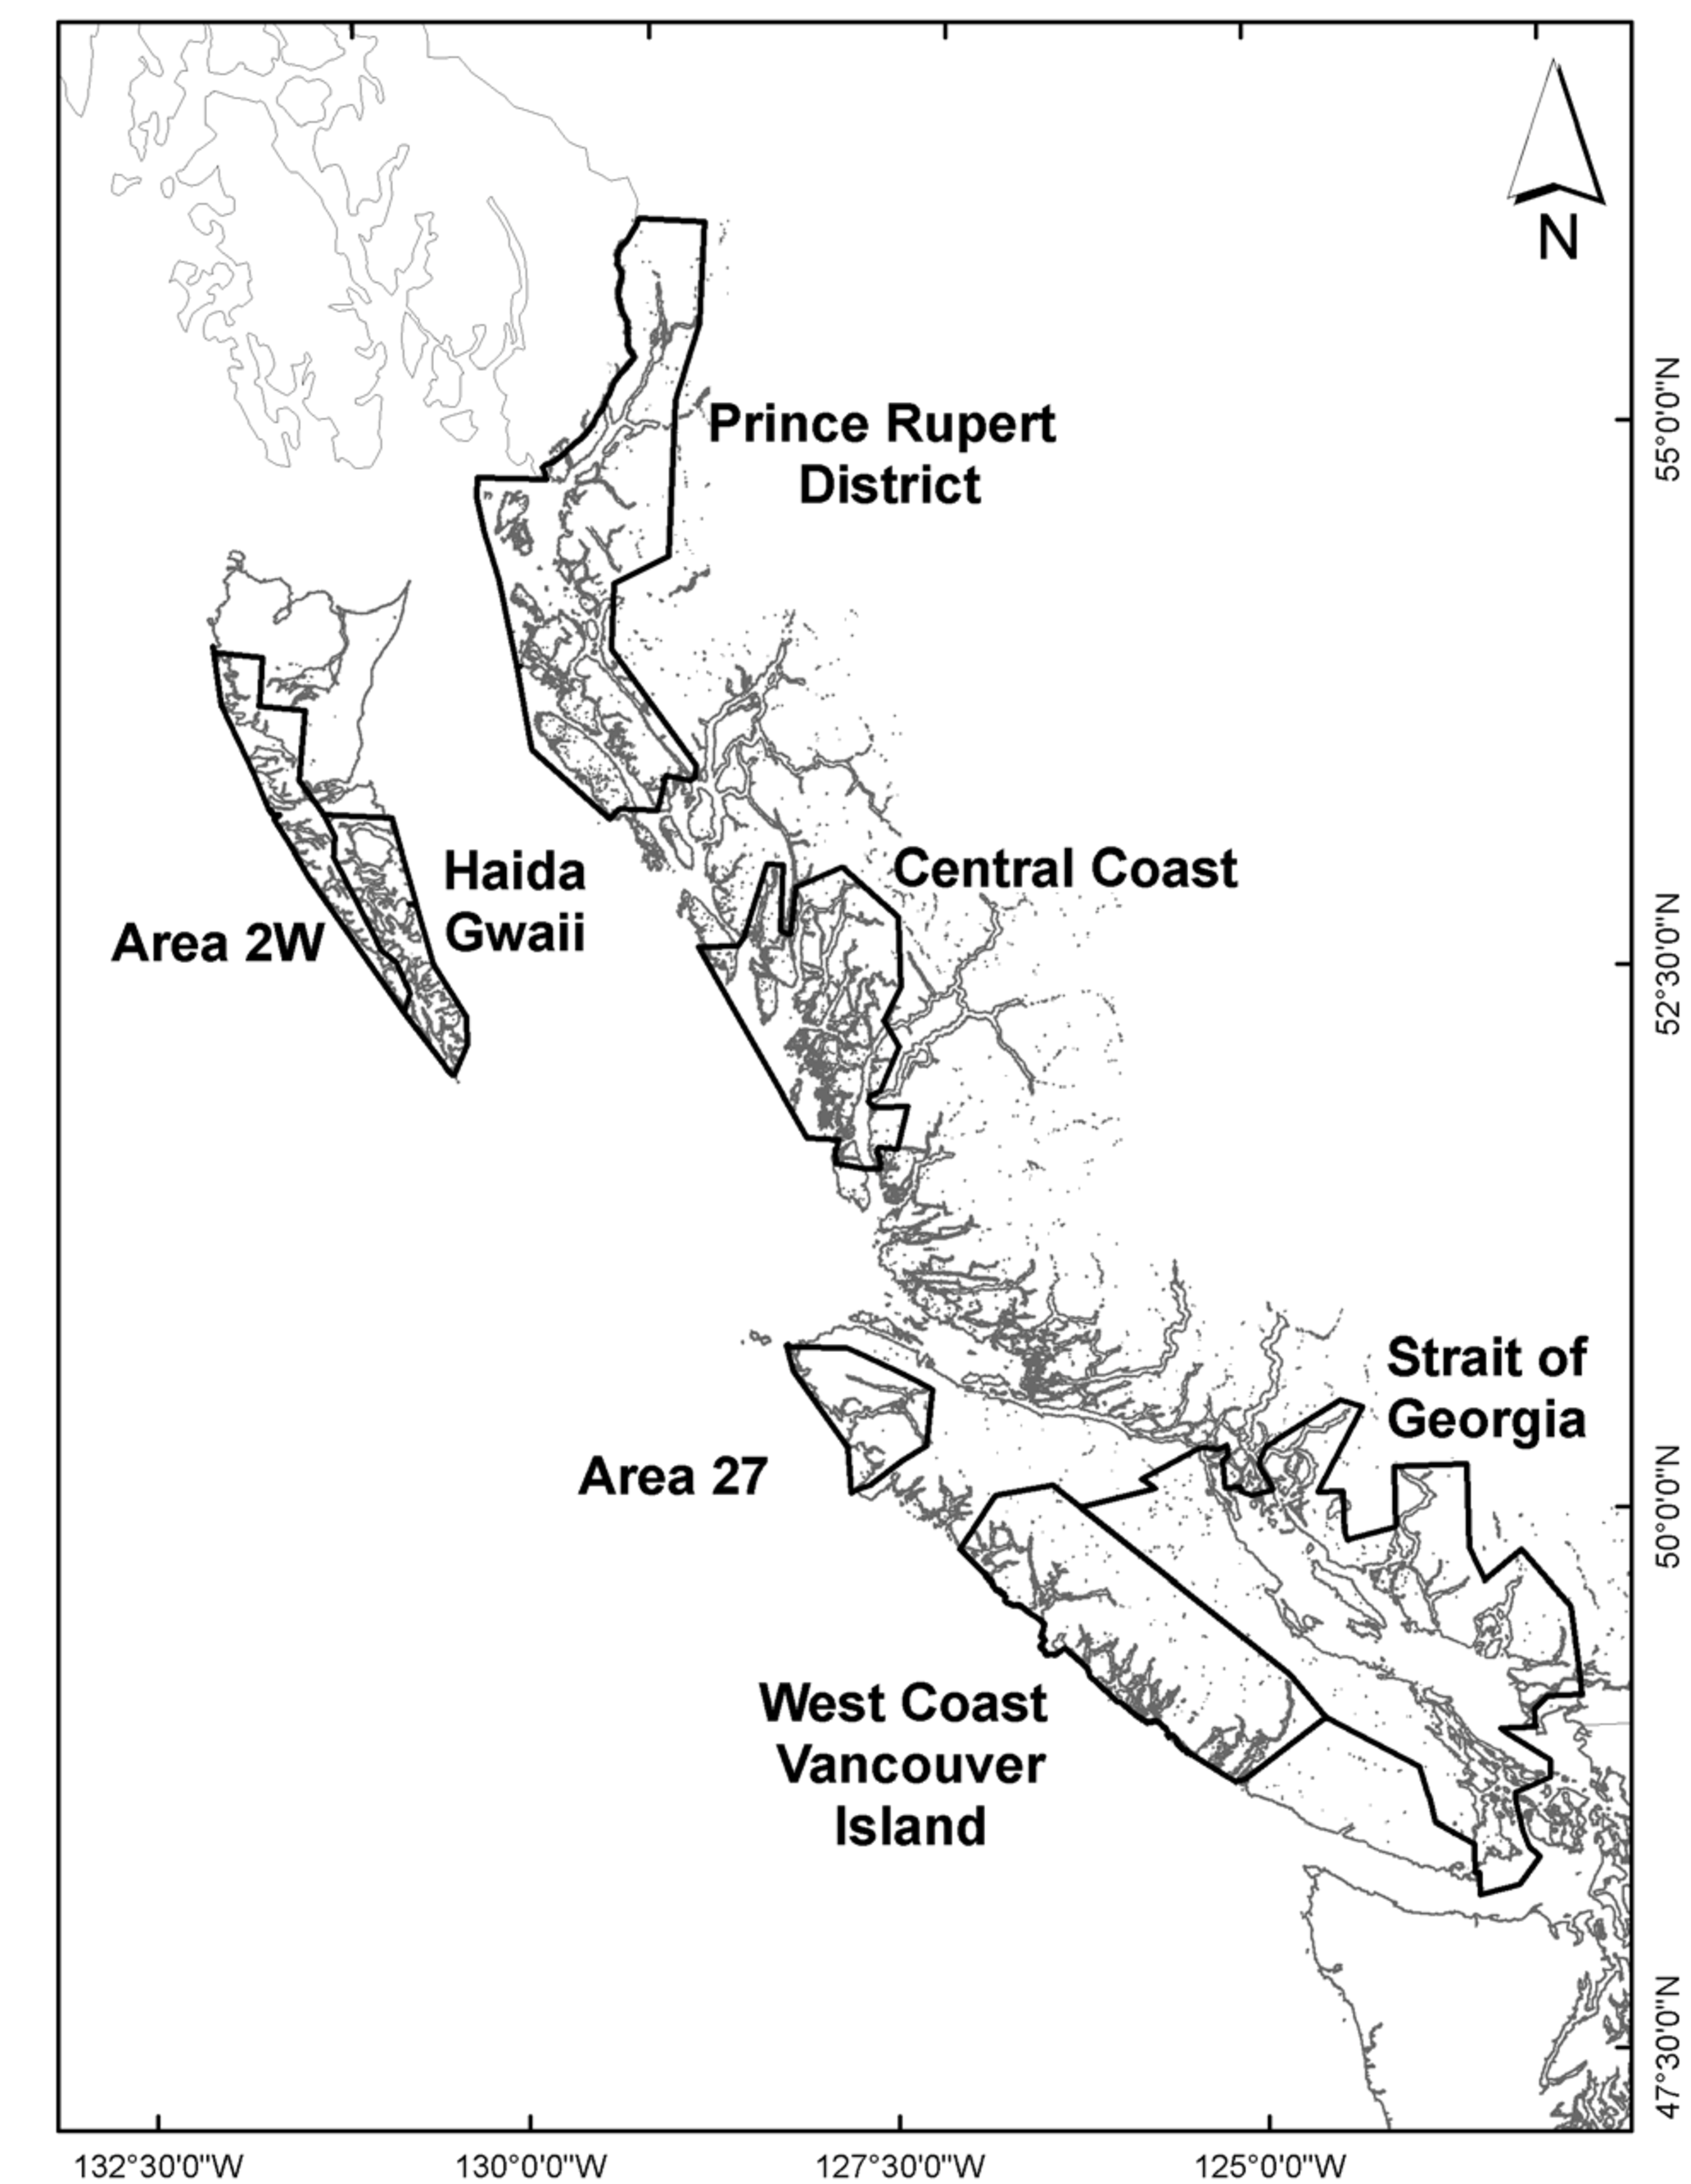
\includegraphics[width=\textwidth]{Figs/HerringAreaMap.pdf}
	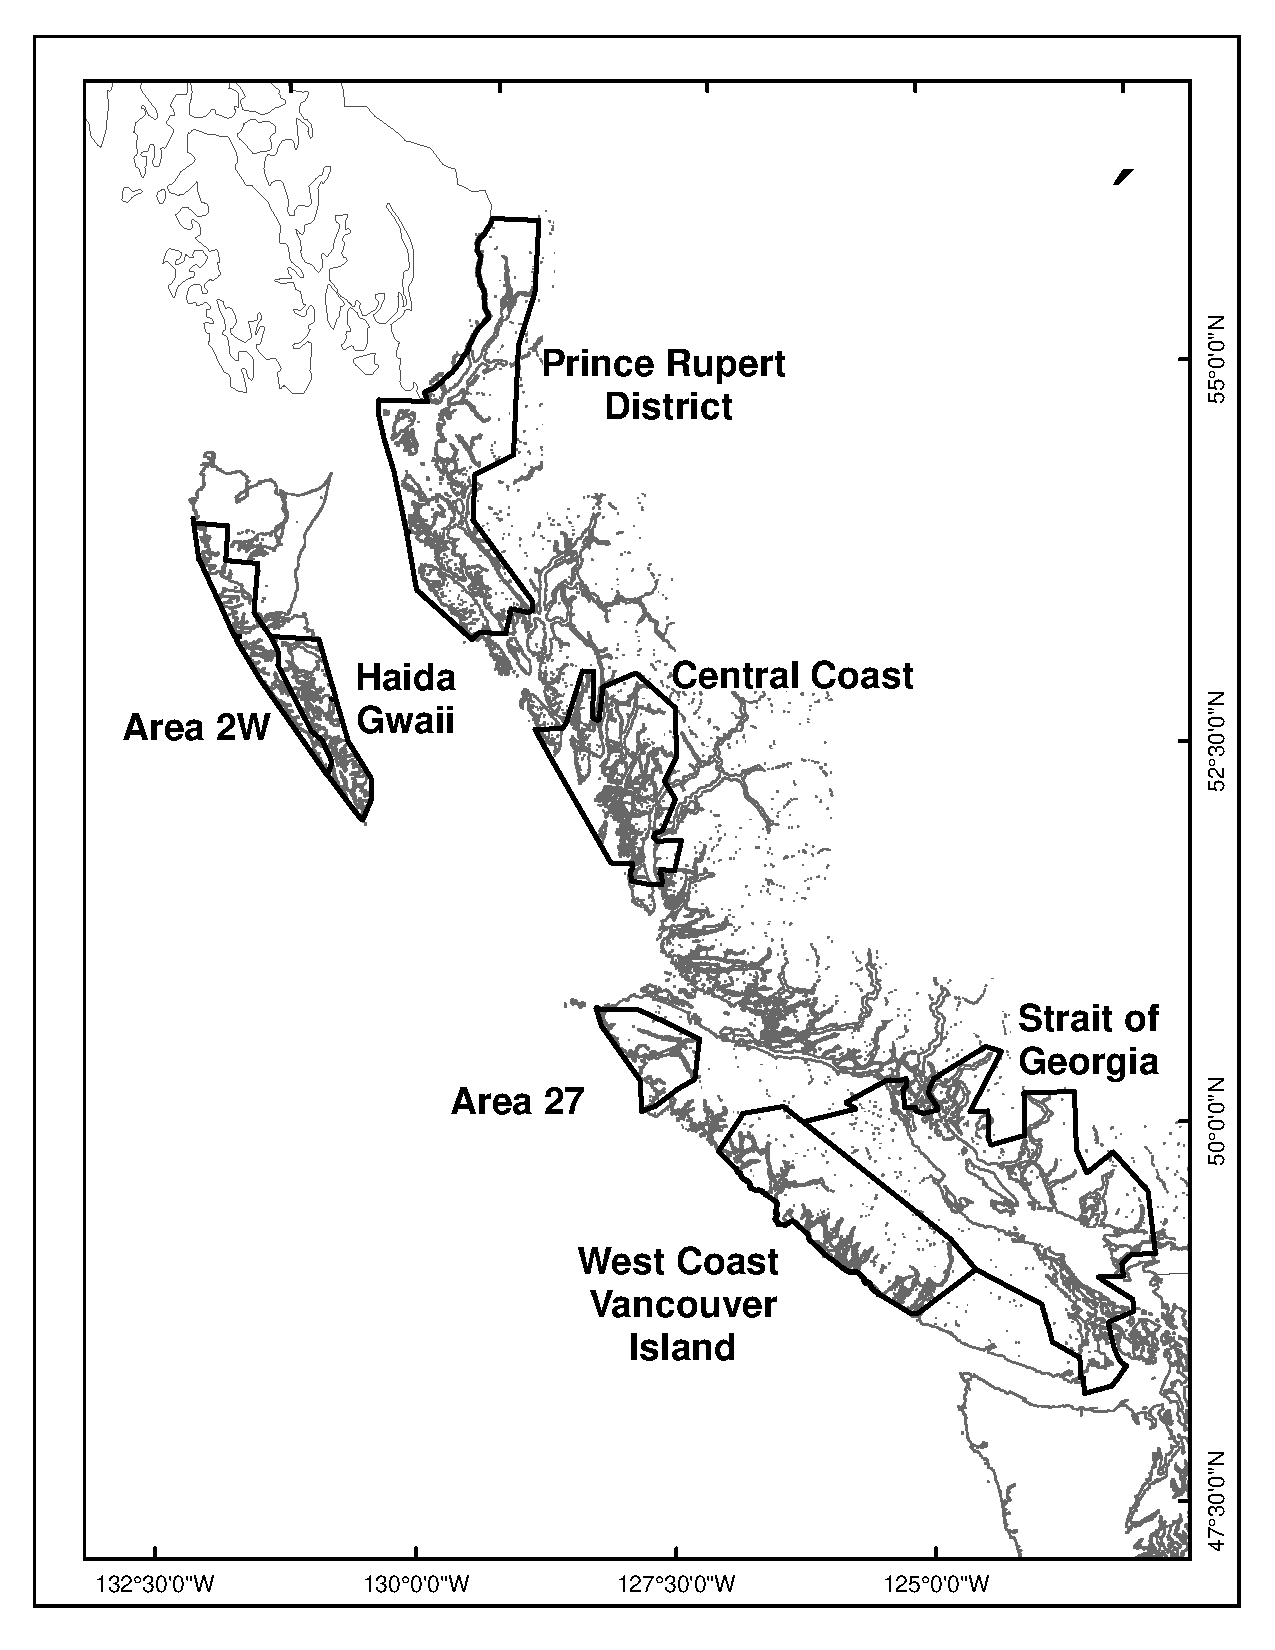
\includegraphics[width=\textwidth]{PBSfigs/Assessment_Regions_2W_27_2010_HG.pdf}
	\caption{B.C. herring major stock areas: Haida Gwaii (HG or QCI 2E), Prince Rupert District (PRD), Central
Coast (CC), Strait of Georgia (SOG), West Coast Vancouver Island (WCVI), and minor stock areas: Area 2W and
Area 27.}\label{Fig1}
\end{figure}
	
%%A reference for splines in selectivities can be found at \cite{aarts2009comprehensive}